
\chapter{Specifiche Progettuali}

L'ecosistema MyGelato è un progetto ampio che si basa sulla cooperazione
tra più elementi fondamentali. Alla base troviamo un backend basato
sul framework Ruby on Rails che implementa le funzionalità di creazione,
gestione e fruizione di contenuti multimediali affiancate da un sistema
e-commerce per la compravendita di coupon digitali. Per poter usufruire
di tali servizi è necessario l'utilizzo di un'applicazione mobile,
chiamata \emph{MyGelato}, disponibile per i sistemi operativi mobile
Apple iOS e Google Android; quest'ultima argomento di questa tesi.\bigskip{}

Essendo l'applicazione Android solo una componente di un più ampio
progetto è essenziale fin dalla prima fase di sviluppo valutare correttamente
e nella loro completezza tutte le specifiche date dall'azienda che
ha commissionato il lavoro e tutte quelle date dalla necessità di
far cooperare l'applicazione con le altre parti del sistema. Si valutano
inizialmente le specifiche strutturali e logiche che determinano le
interazioni principali dell'utente con l'applicativo: navigazione,
design e flussi logici. Questi macro argomenti sono presenti in ogni
singolo componente del sistema e per questo devono essere valutati
prima di iniziare qualsiasi tipo di sviluppo: serve considerare le
interazioni tra i flussi logici e valutare come mantenere coerente
il design all'interno di tutta l'interfaccia utente.\bigskip{}

Fatte queste considerazioni si valuta come implementare una navigazione
che permetta all'utente la scelta delle principali funzioni disponibili
all'interno dell'applicazione: \textit{Acquisto/Utilizzo Coupon},
\textit{Lista Gelaterie Preferite}, \textit{Mappa per la Ricerca},
\textit{Mastro Gelatiere} e \textit{Cambio Tema}. Ogni sezione fa
parte dei due principali flussi logici presenti all'interno dell'applicativo:
quello di marketing digitale che permette l'esplorazione da parte
dell'utente delle gelaterie in una determinata zona geografica e delle
relative promozioni; e quello di e-commerce che permette l'acquisto
online, la gestione, il regalo e l'utilizzo dei coupon gelato resi
disponibili dalle gelaterie del circuito MyGelato.\bigskip{}

Si valutano infine le specifiche tecnologiche richieste sia dall'azienda
che dalla necessaria cooperazione con gli altri elementi del progetto.
Vi deve essere la possibilità di avere un'applicazione multilingua,
con autenticazione tramite social network e compatibile con la maggior
parte dei device Android attualmente sul mercato. Sono di forte impatto
anche alcune scelte a livello di comunicazione con il backend che
indirizza lo sviluppo in una comunicazione bidirezionale tra applicazione
e server tramite API REST e notifiche push. Essenziale poi mantenere
la coerenza tra le due applicazioni mobile sviluppate per le piattaforme
iOS e Android, rispettando in ognuna i propri pattern tipici.

\section{Design}

Il design dell'applicazione è uno degli elementi di maggior risalto:
sviluppato fin nel dettaglio permette di personalizzare anche i componenti
più basilari della \emph{User Interface} (\emph{UI}) come icone, testi
e bottoni. Sono presenti tre font custom che devono essere utilizzati
in situazioni e contesti differenti in modo che possa capire fin dal
primo colpo d'occhio quali siano i messaggi informativi e quali siano
quelli di contorno.\bigskip{}

Altro elemento fondamentale presente in quasi ogni schermata è il
tema dell'applicazione. I temi sono principalmente delle colorazioni
differenti che devono caratterizzare e modificare il \emph{main color}
della UI cambiando anche i testi e le icone in base al fatto di essere
temi chiari o scuri fornendo rispettivamente testi e icone neri o
bianchi. Ogni tema, che deve essere selezionabile a piacimento dall'utente
direttamente da una funzione raggiungibile dalla navigazione principale,
ha come nome un gusto differente di gelato e un proprio set di risorse.\bigskip{}

Le risorse grafiche rese disponibili all'interno delle specifiche
richieste servono a rendere coerente l'interfaccia utente in ogni
suo elemento: fin dall'icona per chiudere una sezione a concludere
con ogni elemento della navigazione principale. Il fatto di avere
un'insieme di risorse ben organizzate è necessario, così da includere
di volta in volta in maniera dinamica immagini in base alla lingua
dell'applicazione e al tema chiaro/scuro.

In figura \ref{fig:Risorse-Design} è possibile vedere alcune delle
immagini presentate per la navigazione principale e alcune icone in
tutte le versioni disponibili rispettivamente per un tema chiaro ed
uno scuro.
\begin{center}
\begin{figure}[H]
\begin{centering}
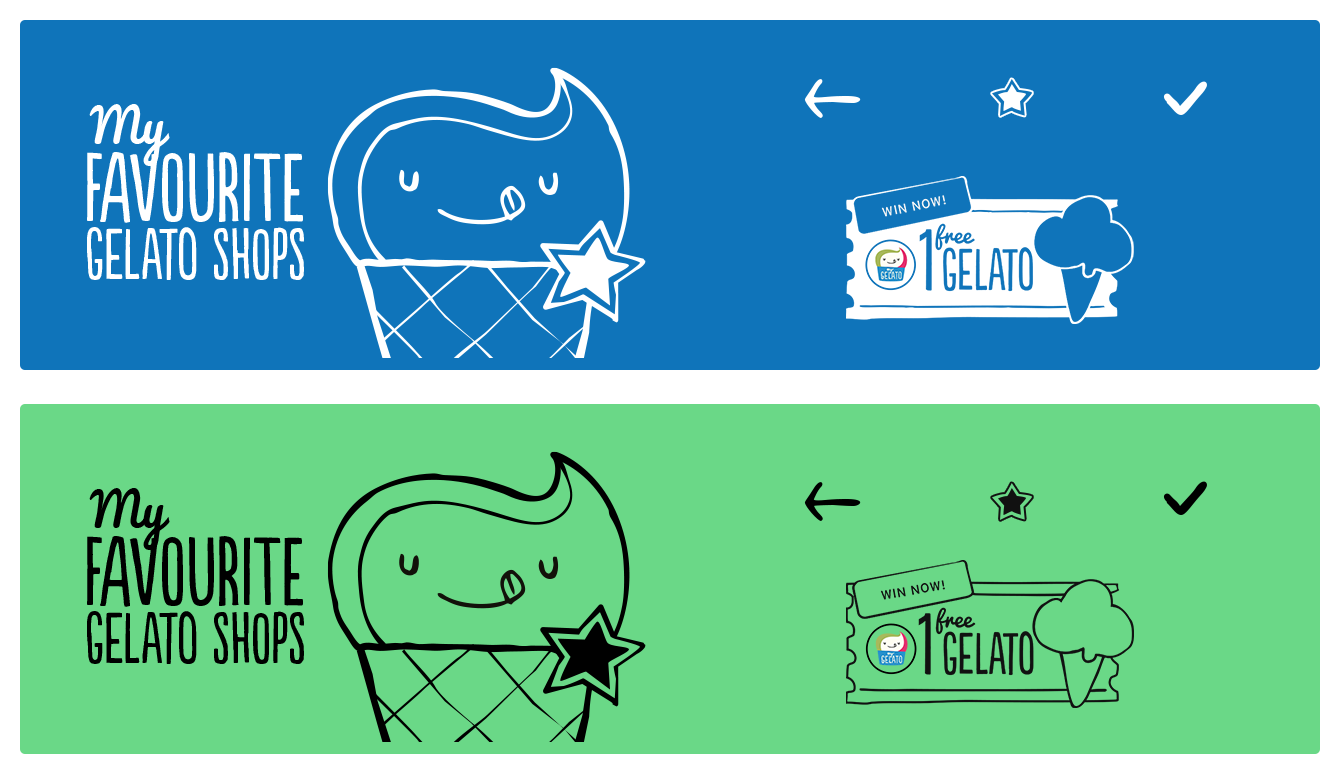
\includegraphics[scale=0.25]{/home/tommaso/Documents/Tesi/thesis/images/res_colors}
\par\end{centering}
\caption{\label{fig:Risorse-Design}Risorse Design}

\end{figure}
\par\end{center}

\section{Ricerca}

L'elemento centrale di tutta l'applicazione è la possibilità di effettuare
una ricerca delle gelaterie, iscritte al circuito MyGelato, presenti
in una determinata zona geografica così da ottenere alcune informazioni
essenziali sull'esercizio e le relative promozioni disponibili. Questa
funzionalità è infatti l'elemento cardine che lega ogni possibile
azione dell'utente all'interno dell'applicazione: è essenziale sia
per il sistema di marketing che per il sistema di e-commerce.\bigskip{}

Ogni utente, anche se non registrato, deve poter accedere a una mappa
che visualizzi tutti gli shop disponibili, sia sotto forma di marker
visibili in base al luogo di ricerca sia sotto forma di lista ordinata
in base alla distanza dall'utente. Ogni elemento, scaricato e aggiornato
in base alle ultime informazioni presenti sul server, permette di
ottenere il nome della gelateria, l'indirizzo e un eventuale recapito
telefonico.

Questo tipo di ricerca permette all'utente di esplorare la zona attorno
al luogo in cui trova, o anche ad un luogo di suo interesse, così
da ottenere informazioni, sia di carattere commerciale sia pubblicitario,
riguardo agli esercizi presenti in maniera molto diretta; permettendo
anche di salvare lo shop all'interno della lista preferiti. Nel frattempo
ogni gelateria presente all'interno del sistema ottiene la possibilità
di essere trovata anche da utenti nuovi che non conoscono la zona
e di pubblicizzarsi tramite una strategia di marketing unificata e
standardizzata: le \emph{carte promozionali}.\bigskip{}

Oltre al sistema di marketing la ricerca delle gelaterie è essenziale
per il sistema di e-commerce poichè la mappa viene utilizzata per
la scelta da parte dell'utente della gelateria per la quale vuole
acquistare un determinato coupon. La ricerca è quindi presente sia
nel sistema di navigazione principale dell'applicazione sia raggiungibile
all'interno di ogni flusso logico scelto dall'utente e come si può
vedere in figura il mockup della mappa permette di capire la necessità
di avere un'implementazione semplice e facilmente utilizzabile da
qualsiasi utente, dove sia possibile passare dalla visualizzazione
a mappa a quella a lista e dove siano già visibili le principali informazioni
riguardo a ogni gelateria.

È possibile osservare in figura \ref{fig:Mockup-Mappa} un mockup
esplicativo per la schermata della ricerca tramite mappa con dettaglio
sulla selezione di un marker informativo.\bigskip{}

\begin{figure}[H]
\begin{centering}
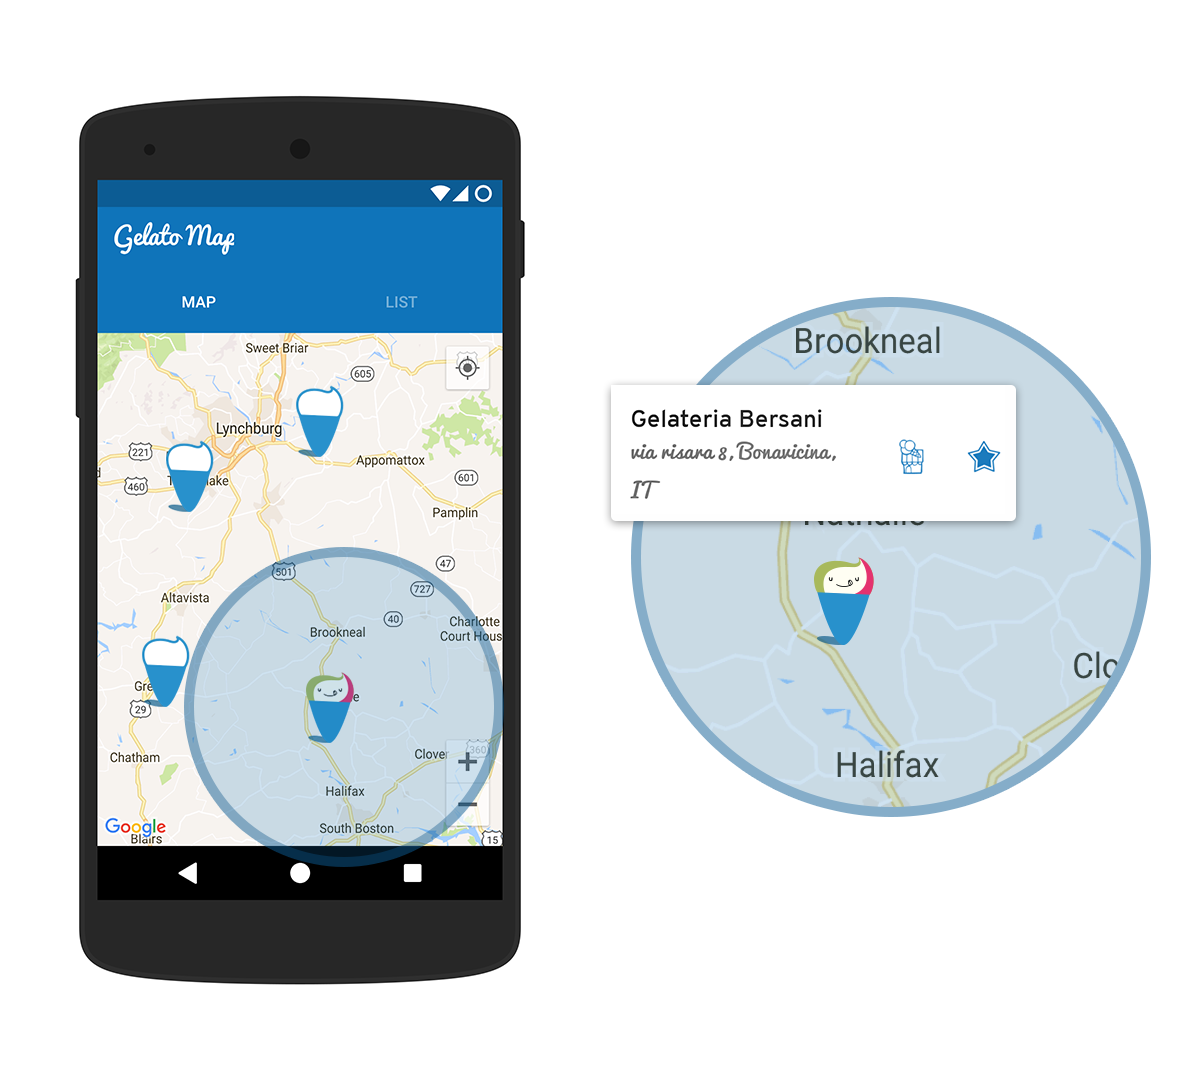
\includegraphics[scale=0.25]{/home/tommaso/Documents/Tesi/thesis/images/mockup_map}
\par\end{centering}
\caption{\label{fig:Mockup-Mappa}Mockup Mappa}

\end{figure}


\section{Utente}

La piattaforma MyGelato per poter offrire alcune funzionalità personalizzate
al singolo utente implementa un sistema di registrazione e di autenticazione.
Questa scelta progettuale è ovviamente fondamentale da considerare
durante lo sviluppo dell'applicazione mobile poichè si deve considerare
un'intera sezione che dia la possibilità all'utente di registrarsi,
modificare parte delle proprie informazioni salvate sul server ed
eseguire il login sulla piattaforma.

Sarà necessario poter accedere direttamente dalla navigazione principale
alle informazioni riguardanti il proprio stato di accesso alla piattaforma,
verificando se si è già autenticati o meno. Le funzionalità che devono
essere più facilmente accessibili sono quindi quelle di login e di
logout, in modo che l'utente in pochi passaggi possa accedere o rimuovere
i propri dati dal dispositivo utilizzato.\bigskip{}

I nuovi utenti potranno utilizzare un form per iscriversi alla piattaforma
MyGelato inserendo solo alcune informazioni essenziali come nome,
cognome, email e password. Le funzionalità di registrazione si basano
principalmente sull'inserimento manuale di un indirizzo di posta elettronica
come metodo identificativo dell'utente, ma deve essere possibile anche
eseguire la registrazione al servizio tramite social network. Il sistema
prenderà in automatico i dati di cui necessita per inserire l'utente
all'interno del proprio database e ogni volta l'accesso all'applicazione
sarà legato al login sui social network.\bigskip{}

All'interno della schermata di login, nel caso vi sia stata una registrazione
manuale, deve essere possibile accedere ad una sezione che permetta
di ricevere nuovamente la password legata all'account sulla email
inserita durante la registrazione. Infine i dati inseriti che non
vengono utilizzati per identificare l'utente potranno essere modificati
una volta effettuato l'accesso direttamente dalla sezione utente.

\section{Marketing Digitale}

Uno dei due \emph{workflow} principali presenti all'interno dell'applicazione
riguarda il marketing digitale che viene svolto per le gelaterie legate
all'ecosistema MyGelato. Ha lo scopo di rendere più facile la ricerca
delle gelaterie, sponsorizzarne eventuali promozioni e permettere
a ogni utente di salvare gli esercizi preferiti così da rimanere aggiornato
sulle nuove promozioni disponibili.

Queste funzionalità, disponibili in buona parte per qualsiasi utente
anche non registrato, seguono un flusso logico che parte dalla ricerca
degli shop e trova effetto principale nella scoperta e nell'utilizzo
delle carte promozionali, della singola gelateria e del Mastro Gelatiere.

\subsection{Carte Promozionali}

Le carte promozionali sono il principale mezzo di advertising all'interno
dell'applicazione: sono dei volantini digitali formati da un'immagine
o un video, un titolo, un testo descrittivo, un eventuale recapito
telefonico e un link per ottenere maggiori informazioni riguardo alla
promozione in oggetto. Ci sono due tipologie di carte: le carte specifiche
di ogni esercizio, ovvero i volantini informativi della singola gelateria,
e le carte del mastro gelatiere che invece si rifanno alle promozioni
generiche proposte per l'intero sistema.\bigskip{}

Le carte della singola gelateria altro non sono che le ultime promozioni
legate all'attività: sconti, novità, messaggi informativi. L'utente
in questo modo può facilmente reperire le informazioni pubblicitarie
di una determinata gelateria online e in mobilità; considerando che
difficilmente in questo campo vi è già una diffusa pubblicizzazione
sui social network o sui sistemi di advertising. Ogni shop iscritto
al circuito MyGelato ha quindi la possibilità di ottenere una maggior
copertura pubblicitaria tramite l'utilizzo di un sistema centralizzato
e standardizzato.

Le carte di uno stesso esercizio devono essere raggruppate in modo
che l'utente possa scorrerle e visualizzare tutte le promozioni o
informazioni disponibili insieme. La schermata per questa visualizzazione
deve essere raggiungibile ogni volta che sono mostrate le informazioni
della gelateria: sia internamente alla ricerca che nella lista dei
preferiti dell'utente.\bigskip{}

Oltre alle singole gelaterie l'ecosistema MyGelato prevede anche le
carte del Mastro Gelaterie che comprendono promozioni, informazioni
e novità pubblicate genericamente dagli amministratori del sistema
e che sono valide per tutti gli esercizi facenti parte del circuito.
Essendo un insieme di carte totalmente generiche, quindi slegate da
qualsiasi flusso logico, e di fondamentale importanza per il sistema
di advertising creato, questa sezione deve essere inserita all'interno
della navigazione principale del sistema.\bigskip{}

Infine, come avverrà poi per le gelaterie preferite, ogni utente registrato
dovrà avere la possibilità di essere notificato di eventuali nuove
promozioni nel momento stesso in cui diventeranno disponibili.

\subsection{Preferiti}

La gestione delle proprie gelaterie preferite è uno degli elementi
presenti all'interno della navigazione principale dell'applicazione,
accessibile da qualsiasi utente anche non registrato: permette di
salvare sul proprio dispositivo gli esercizi di maggiore interesse.

Questo dà modo all'utente di poter accedere in ogni momento, specialmente
in mobilità, alle informazioni che più gli interessano di ogni gelateria:
indirizzo, recapito telefonico ed eventuali promozioni. La ricerca
in questo caso è molto semplificata poichè viene presentata una sezione
a parte con una lista degli shops preferiti, senza dover obbligare
l'utente a effettuare una nuova ricerca all'interno della mappa. Il
salvataggio all'interno dei preferiti avviene direttamente all'interno
della ricerca, sia tramite la mappa che tramite la lista grazie a
un'icona esemplificativa.\bigskip{}

Questa funzionalità è pensata principalmente per fidelizzare il consumatore:
ogni utente avendo la possibilità di salvare una gelateria ha anche
la possibilità di ottenere velocemente informazioni su nuove promozioni,
trovare velocemente i contatti dell'esercizio come se li avesse salvati
in rubrica e valutare ogni volta la distanza tra se e lo shop.\bigskip{}

Il passo successivo in questo senso è dato dal rendere bidirezionale
questo collegamento, rendendo in alcuni casi non necessaria la ricerca
da parte dell'utente di nuove informazioni fornendogliele invece a
ogni aggiornamento. Per fare questo, solo nel caso di utenti registrati,
l'aggiunta di uno shop ai preferiti include le funzionalità di geofencing
e notifiche push, quest'ultima presente anche per le carte promozionali
del mastro gelatiere.

Il geofencing permette di ricevere una notifica ogni qualvolta l'utente
si trovi a meno di 5 km da una delle proprie gelaterie, così da essere
informato di essere vicino in termini di localizzazione. Le notifiche
push invece sono attivate per avvertire un utente che una delle proprie
gelaterie ha pubblicato una nuova promozione tramite l'aggiunta una
carta sul sistema MyGelato. L'utente così rimane informato costantemente
delle ultime promozioni disponibili e il proprietario di una gelateria
ha la certezza di effettuare pubblicità diretta tra se e i suoi clienti
più affezionati.

\section{E-Commerce}

Il secondo flusso logico presente all'interno dell'applicazione riguarda
l'acquisto e l'utilizzo di coupon gelato online e in completa mobilità.
Questo sistema già più che diffuso in tantissimi altri ambiti della
vendita online è uno dei cardini su cui maggiormente si vuole puntare
sia per funzionalità sia per innovazione.\bigskip{}

I \emph{Coupon} gelato sono buoni acquisto che si possono acquistare
direttamente tramite l'applicazione e permettono a chiunque ne sia
virtualmente in possesso di utilizzarli nelle gelaterie che li hanno
rilasciati tramite validazione. L'acquisto dei buoni deve poter essere
fatto in qualsiasi momento utilizzando le ultime tecnologie disponibili
per i pagamenti online; essenziale mantenere un occhio di riguardo
alla sicurezza di questo tipo di transizioni.\bigskip{}

Tra le specifiche risulta essere presente anche il concetto di condivisione
dei coupon tramite un sistema di \emph{share/redeem}: un utente che
ha acquistato un coupon ha la possibilità di condividerlo con un altro
utente registrato alla piattaforma che può riscuotere poi il buono.
La condivisione deve avvenire tramite applicazioni e canali di comunicazioni
facilmente utilizzabili all'interno di uno smartphone.\bigskip{}

Infine vi deve essere ovviamente la possibilità di validare un coupon
una volta che si decide di utilizzarlo all'interno della gelateria
che lo ha rilasciato online tramite il circuito MyGelato. Questo procedimento
prevede due entità in gioco, colui che possiede il coupon e il gelataio
che deve poterlo validare; in entrambi i casi le funzionalità da implementare
dovranno essere presenti all'interno dell'applicazione in base al
tipo di account utilizzato così da mantenere coerenza negli strumenti
utilizzati per collegarsi alla piattaforma.

\subsection{Coupon}

I Coupon sono buoni per l'acquisto di un bene materiale, normalmente
gelati, che si può ritirare in qualsiasi momento in sede all'esercizio
che ha effettuato la vendita. Hanno un nome e un valore, il prezzo,
scelti durante l'inserimento tramite il sistema amministrativo gestionale
che può inserire anche informazioni aggiuntive come la scadenza e
la valuta. Sono generici per tutto l'ecosistema e sono quindi disponibili
per ogni gelateria facente parte del circuito MyGelato anche se all'acquisto
sarà necessario specificare l'esercizio nel quale si desidereranno
poi utilizzare.\bigskip{}

All'interno della navigazione principale dell'applicazione sarà necessario
avere una sezione apposita per poter gestire tutti i propri coupon:
una lista di quelli utilizzati, quelli regalati ad altri utenti e
quelli che si possono ancora utilizzare personalmente. Questa sezione
sarà disponibile offline ma dovrà ogni volta essere sincronizzata
con il server in modo da avere coerenza anche utilizzando la stessa
applicazione con lo stesso account da dispositivi differenti.\bigskip{}

Oltre alla possibilità di acquistare coupon si dovrà poter accedere
direttamente alle funzioni di condivisione, riscatto e utilizzo così
da avere una gestione centralizzata di tutto il flusso logico legato
all'e-commerce.

\subsection{Acquisto}

L'acquisto di un coupon è permesso a qualsiasi utente che si sia registrato,
tramite mail o social network, al circuito MyGelato. Questa funzionalità
è raggiungibile direttamente tramite parte della navigazione principale
dell'applicazione, anche se deve essere disponibile solo nel caso
in cui l'utente abbia eseguito il login, altrimenti dovranno essere
richieste le credenziali di accesso.\bigskip{}

Le operazioni richieste per l'acquisto di un coupon dovranno essere
tutte racchiuse all'interno di una stessa schermata in cui l'utente
verrà guidato attraverso le varie fasi fino all'avvenuta transizione.
Il primo passo da svolgere è la scelta della gelateria su cui eseguire
l'acquisto, come spiegato precedentemente si andrà a sfruttare la
mappa e la lista per la ricerca degli shop già utilizzata all'interno
di altre funzionalità. In questo caso però verranno visualizzati solo
le gelaterie che permettono l'acquisto di coupon e quando verranno
selezionati i marker non si otterranno tutte le informazioni sull'esercizio
ma sarà presente un'icona per selezionare lo shop.\bigskip{}

Una volta selezionata la gelateria dovranno essere scaricati dal server
i coupon disponibili e nel frattempo verrà resa disponibile la scelta
del metodo di pagamento che si appoggerà ad un sistema di pagamento
online esterno. Si potrà scegliere tramite una lista di metodi di
pagamento quello che si preferirà usare che sarà successivamente impostato
come predefinito.

Scelto il metodo di pagamento, scorrendo la lista dei coupon disponibili
ed decidendo il valore che si vuole acquistare si potrà infine scegliere
di completare l'acquisto che in caso di successo dovrà poi riportare
l'utente sulla sezione di gestione dei coupon e altrimenti presentare
un messaggio di errore.

\subsection{Condivisione e Riscatto}

Le funzionalità di condivisone e riscatto che si vogliono implementare
all'interno dell'applicazione rendono importante capire come far dialogare
due dispositivi differenti in modo che abbiano informazioni coerenti
uno con l'altro e in modo che sia semplice l'utilizzo da parte di
utenti non esperti. Per rendere questa funzionalità accessibile da
chiunque si dovrà legare ogni coupon grazie ad un codice alfanumerico
di sei cifre detto PNR (\emph{Product Nr.}) che potrà quindi essere
condiviso tramite qualsiasi mezzo disponibile.\bigskip{}

L'uso di un codice inviabile facilmente come teso permette di sfruttare
altri applicativi presenti sul dispositivo dell'utente per la condivisione
tra persone differenti. Scegliendo il coupon da regalare si dovrà
quindi chiedere all'utente tramite quale canale di comunicazione preferisce
inviare il codice PNR per poi inserire il codice in un testo promozionale
legato ad un link di reindirizzamento a una pagina web della piattaforma
MyGelato.

L'inserimento del link a una pagina web della piattaforma accessibile
online da qualsiasi dispositivo è una funzionalità di grande potenza:
nel caso in cui la pagina web sia raggiunta da un dispositivo che
ha installato sopra l'applicazione MyGelato aprirà direttamente l'applicativo
stesso gestendo internamente il codice presente; altrimenti verrà
presentata una pagina web che suggerisce all'utente di scaricare l'applicazione
dai principali store mobile.\bigskip{}

Valutato come scegliere di condividere un coupon è necessario inserire
una funzione all'interno dell'applicazione che ne permetta il riscatto
tramite il solo inserimento del codice PNR. Raggiungibile dalla navigazione
principale vi sarà una sezione che permetta di eseguire questa operazione
in maniera molto semplice e che, nel caso venga avviata l'applicazione
tramite la gestione del link web di cui si è parlato precedentemente
sarà compilata in automatico.

Tramite un semplice controllo sul server verrà quindi controllato
se l'utente può riscattare il codice e le informazioni saranno aggiornate
per entrambi gli utenti: chi ha regalato il coupon e chi invece può
utilizzarlo.

\subsection{Utilizzo e Validazione}

L'ultimo passo all'interno del flusso logico di questo sistema di
e-commerce è ovviamente l'utilizzo e la validazione di un coupon per
acquistare un bene materiale direttamente in sede all'esercizio che
ha venduto il buono. Per semplificare l'utilizzo della piattaforma
MyGelato ci si è rifatti nuovamente al fatto che gli smartphone siano
diventati dei beni di uso comune e che quindi anche i proprietari
delle gelaterie possano utilizzare l'applicazione MyGelato come mezzo
per la validazione dei coupon.\bigskip{}

Allo stesso modo che per le funzionalità di condivisone e riscatto
si è scelto di utilizzare i codici PNR dei coupon come mezzo per far
dialogare i due dispositivi di chi vuole utilizzare un buono e di
chi deve verificare che sia valido. Rispetto ad un sistema di condivisione
che prevede la presenza di un canale di comunicazione personale tra
i due utenti si dovrà valutare l'utilizzo di mezzi più semplici e
slegati.

Si è quindi proposto di generare un QR Code a partire dal codice PNR
di ogni coupon, raggiungibile direttamente cliccando sul buono presente
nella lista di gestione interna all'applicazione. Il consumatore dovrà
quindi mostrare il QR Code al proprietario dell'esercizio che, utilizzando
la stessa applicazione MyGelato con un account di tipo \emph{gelatiere},
utilizzerà una funzione di validazione tramite lettura del codice
mostrato. Sarà infine necessaria una connessione al server da parte
di entrambi i dispositivi per verificare l'avvenuta validazione del
coupon così da procedere all'acquisto materiale del bene rappresentato
dal buono.

\newpage{}
